\documentclass[10pt]{article}
\usepackage{fullpage}
\usepackage{graphicx}
\newcommand{\tab}{\hspace*{2em}}
\begin{document}
	\begin{flushright}
	Lindsey Bieda and Joe Frambach\\
	Greedy Algorithm Problems\\
	9.11.2011
	\end{flushright}
	\noindent
	9.  The input to this problem consists of an ordered list of $n$ words. The length of the $i$th word is $w_{i}$, that
			is the $i$th word takes up $w_{i}$ spaces.  (For simplicity assume that there are no spaces between words.)
			The goal is to break this ordered list of words into lines, this is called a layout. Note that you can not
			reorder the words.  The length of a line is the sum of the lengths of the words on that line. The ideal
			line length is $L$. No line may be longer than $L$, although it may be shorter.  The penalty for having a
			line of length $K$ is $L - K$. \textit{The total penalty is the \textbf{sum} of the line penalties}. The problem is to find a
			layout that minimizes the total penalty.\\
			Prove of disprove that the following greedy algorithm correctly solves this problem.
			
			\begin{verbatim}
			For i= 1 to n
			     Place the ith word on the current line if it fits
			      else place the ith word on a new line
			\end{verbatim}
			% answer here
			Prove that the greedy algorithm is correct.\\
			Proof: Assume $\exists$ input I $\ni$ GRE(I) $<$ OPT(I), let OPT be the optimal solution that agrees with greedy
			for the most steps, $k$.\\
			\\
			$GRE(I) = 
			\begin{array}{ccccc}
				w_{0} & w_{1} & \ldots & w_{k-1} & w_{k}\\
				w_{k+1} & w_{k+2} & \ldots & w_{n}\\  
			\end{array}\bigg\}, k = N L - \sum w$, where N is the number of lines
			\\
			\\
			$OPT(I) = 
			\begin{array}{ccccc}
				w_{0} & w_{1} & \ldots & w_{k-1}\\
				w_{k} & w_{k+1} & \ldots & w_{n-1}\\
				w_{n}  
			\end{array}\bigg\}, k = N L - \sum w$\\
			Let the first point of disagreement be at point $k$. We can construct $OPT^{\prime}$ as the following.\\
			$OPT^{\prime}(I) = 
			\begin{array}{ccccc}
				w_{0} & w_{1} & \ldots & w_{k}\\
				w_{k+1} & w_{k+2} & \ldots & w_{n-1}\\
				w_{n}  
			\end{array}\bigg\}, k = N L - \sum w$\\
			\\
			At this point $k$ is non-increasing, so $OPT^{\prime} \geq OPT$, and we can construct $OPT^{\prime\prime}$ which
			will agree with greedy for an additional step.\\
			\\
			$OPT^{\prime\prime}(I) = 
			\begin{array}{ccccc}
				w_{0} & w_{1} & \ldots & w_{k}\\
				w_{k+1} & w_{k+2} & \ldots & w_{n}
			\end{array}\bigg\}, k = (N - 1) L - \sum w$\\
			\\	
			$OPT \leq OPT^{\prime} \leq OPT^{\prime\prime} \leq \ldots = GRE \bot$\\
			\\				
			\newpage
			\noindent	 
	10. The input to this problem consists of an ordered list of $n$ words. The length of the $i$th word is $w_{i}$ , that
			is the $i$th word takes up $w_{i}$ spaces.  (For simplicity assume that there are no spaces between words.)
			The goal is to break this ordered list of words into lines, this is called a layout. Note that you can not
			reorder the words.  The length of a line is the sum of the lengths of the words on that line. The ideal
			line length is $L$. No line may be longer than $L$, although it may be shorter.  The penalty for having a
			line of length $K$ is $L - K$. The total penalty is the maximum of the line penalties. The problem is to
			find a layout that minimizes the total penalty.\\
			Prove of disprove that the following greedy algorithm correctly solves this problem.
			
			\begin{verbatim}
			For i= 1 to n
			     Place the ith word on the current line if it fits
			       else place the ith word on a new line
			\end{verbatim}
			%answer here
			Counter-example:\\
			Consider the following input: $I$ = [2, 1, 1] and $L$ = 3,\\
			GRE(I) = $
			\begin{array}{ccc}
				2 & 1 & k = 0\\
				1 &   & k = 2\\
				  &   & max(k) = 2
			\end{array}$
			\\
			\\
			\\
			OPT(I) = $
			\begin{array}{ccc}
				2 &   & k = 1\\
				1 & 1 & k = 1\\
				  &   & max(k) = 1
			\end{array}$\\
			\\			
			\newpage
			\noindent
	13. Consider the following problem.\\
			INPUT: Positive integers $r_{1}, \ldots, r_{n}$ and $c_{1}, \ldots , c_{n}$.\\
			OUTPUT: An $n$ by $n$ matrix $A$ with 0/1 entries such that for all $i$ the sum of the $i$th row in $A$ is $r_{i}$
			and the sum of the $i$th column in $A$ is $c_{i}$, if such a matrix exists.\\
			Think of the problem this way.  You want to put pawns on an $n$ by $n$ chessboard so that the $i$th row
			has $r_{i}$ pawns and the $i$th column has $c_{i}$ pawns.\\
			Consider the following greedy algorithm that constructs $A$ row by row.  Assume that the first $i - 1$
			rows have been constructed. Let a $j$ be the number of 1�s in the $j$th column in the first $i - 1$ rows. Now
			the $r_{i}$ columns with a maximum $c_{j} - a_{j}$ are assigned 1�s in row $i$, and the rest of the columns are
			assigned 0�s. That is, the columns that still needs the most 1�s are given 1�s. Formally prove that this
			algorithm is correct.\\
			\\
			%answer here
			Assume $\sum r_{1}, \ldots, r_{n} = \sum c_{1}, \ldots , c_{n}$ otherwise it is \textsc{\texttt{\textsl{\textit{\textbf{NOT}}}}} correct.\\
			\\
			Prove that the greedy algorithm is correct.\\
			Proof: Assume $\exists$ input I $\ni$ GRE(I) $<$ OPT(I), let OPT be the optimal solution that agrees with greedy
			for the most steps, $k$.\\
			$k$, in this case, represents a position in the matrix $I$, $(k_x,k_y)$.
			\\
\begin{figure}[h]
	\centering
		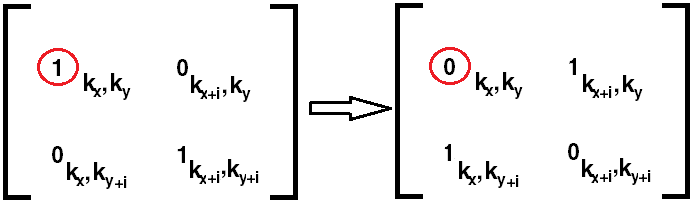
\includegraphics[width=450px]{greedy13fig1.png}
	  \caption{There must exist corresponding nodes in this configuration.}
\end{figure}
			\\
			\\
			There must exist corresponding nodes in the configuration shown above (Fig.1). We can show that this must be the case.
			\\
\begin{figure}[h]
	\centering
		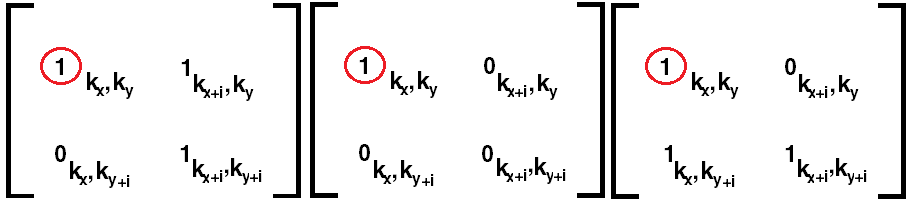
\includegraphics[width=450px]{greedy13fig2.png}
	  \caption{In each of these cases, swapping the values results in an incorrect solution}
\end{figure}
			\\
			There are seven cases to consider if the configuration is not found. In each of these cases (Fig. 2), swapping the values
			results in an incorrect solution. So the configuration (Fig.1) must exist.\\
			\\
			$OPT^\prime$ is constructed by flipping the values in each node $[(k_x,k_y), (k_x+i,k_y), (k_x,k_y+i), (k_x+i,k_y+i)]$,
			as demonstrated in Fig. 1. $OPT^\prime$ results in an optimal solution since the sums of the rows and columns remain correct.
	    The same holds true if $(k_x,k_y) = (k_x+i,k_y+i) = 0$ and $(k_x,k_y+i) = (k_x+i,k_y) = 1$.
	    \\
	    We have now constructed an $OPT^\prime$ which agrees with $OPT$ for one more step and is still optimal.\\
	    \\
	    $OPT \leq OPT^{\prime} \leq OPT^{\prime\prime} \leq \ldots = GRE \bot$\\
			\\
\end{document}
	
	